Price of the project!
It depends where u buy arduino, ethernet shields etc. If i didn't add project from other lesson it could be around from 70PLN to 170PLN depends on which website u will buy or in what store. Also the price is the time you have to learn many languages.
\begin{figure}[!h]
	\centering
	
\includegraphics[width=2.5in]{cena.jpg}
	\caption{Price.\label{fig:Cena}}
\end{figure}
\newline
\newline
I gained the ability to program in various languages, to program in markup languages, i.e. html and css, to create graphs on a website with the help of data retrieval from a database.

\begin{figure}[!h]
	\centering
	
\includegraphics[width=2.5in]{skill.png}
	\caption{Skill.\label{fig:Skill}}
\end{figure}
What's next?\newline
1. To fix not working properly server.\newline
2. Maybe do it with only arduino without database.\newline
3. Add some animation on page.\newline
4. Add some other charts maybe do it with real time chart with showing only 20 data points.\newline
5. Improve the website so that it can be used from various devices on the internet.\newline
\newline
\newline
To sum up i learnt a lot of things. I learnt how to program in different languages. Also I gain knowledge to do my project or knowledge useless to my project but maybe usefull in future. Also I improved english skills with writing a raport and making a presentation, I improved my english speach. I learnt how to send data from arduino to database and from database to WebPage. I improved my skills with database. I got experience in making charts on webpages. It was really fun to do the project. Now I have more knowledge and can do other projects or improve my WebPage to better stage.
\begin{figure}[!b]
	\centering
	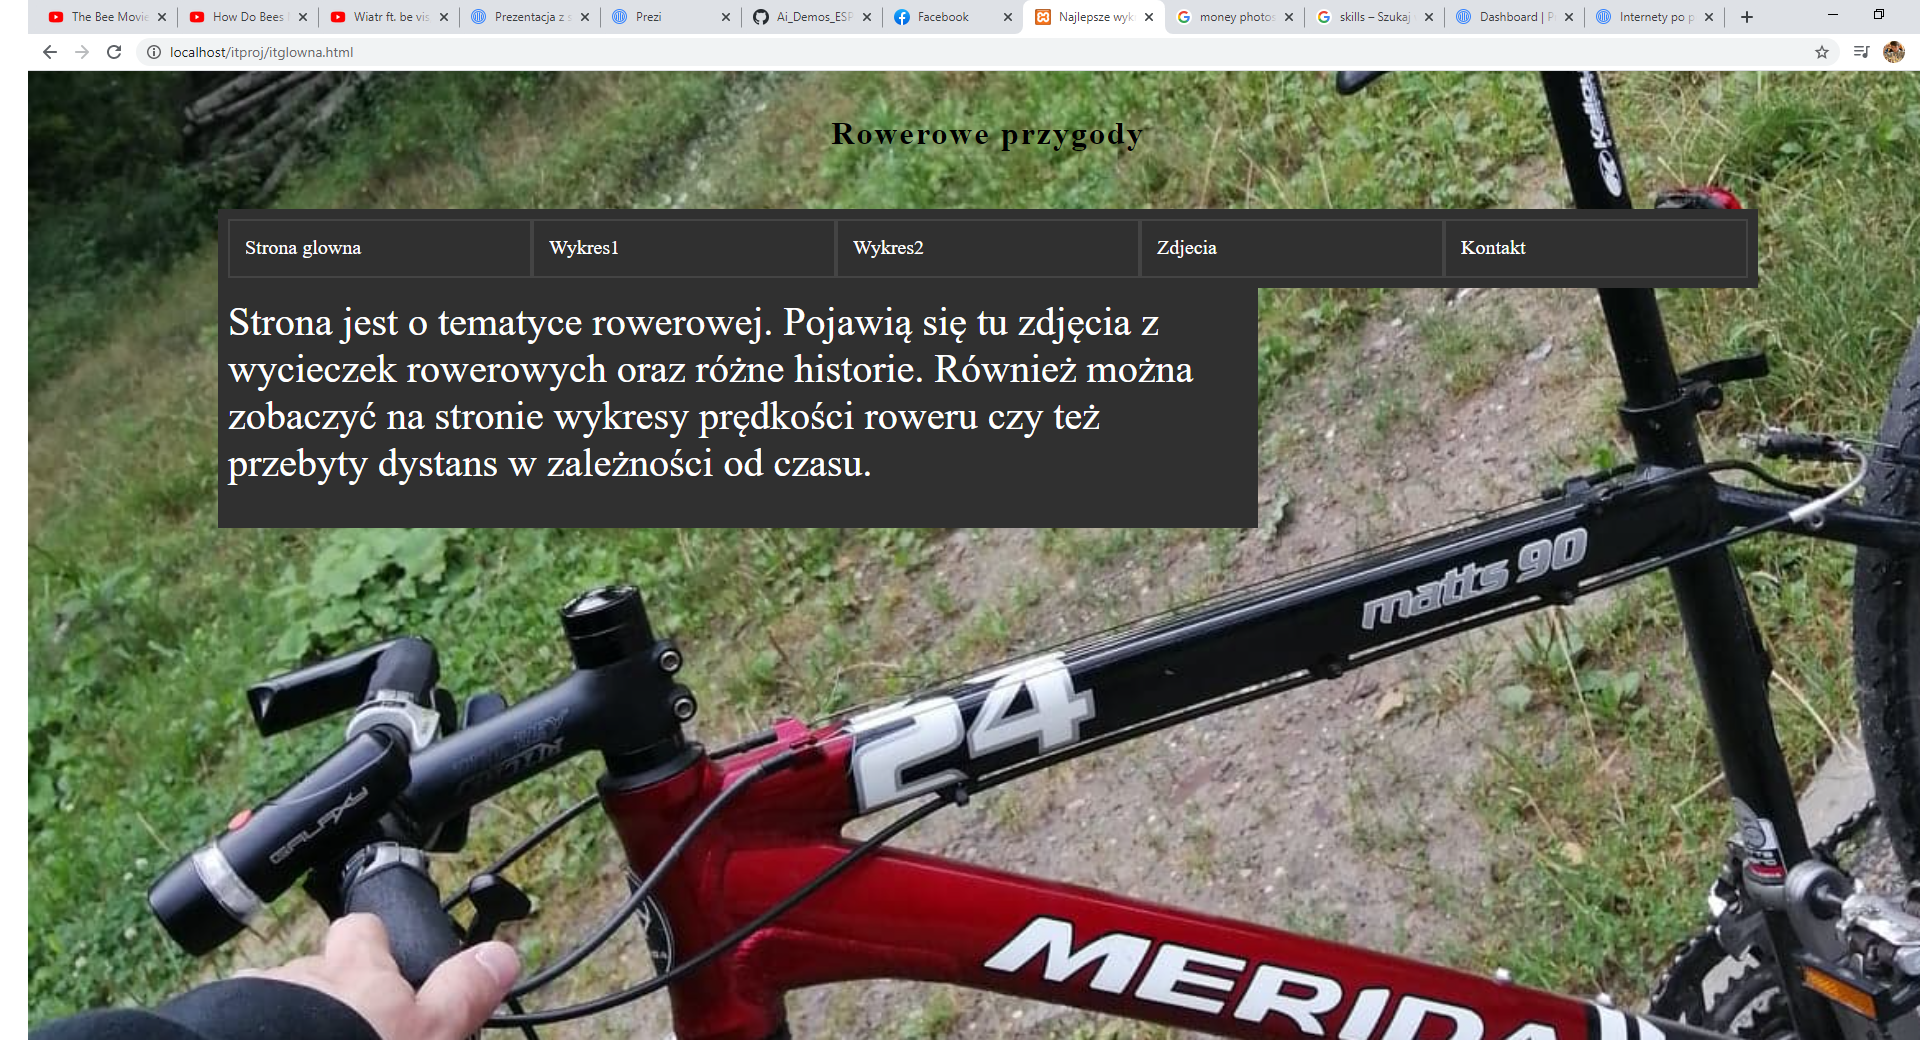
\includegraphics[width=5.0in]{stronaglowna.png}
	\caption{Moja Strona.\label{fig:Stronaglowna}}
\end{figure}
\newline
On the end i can add photo with my arduino and how arduCam with build esp in it look like.\newline

\begin{figure}[!b]
	\centering
	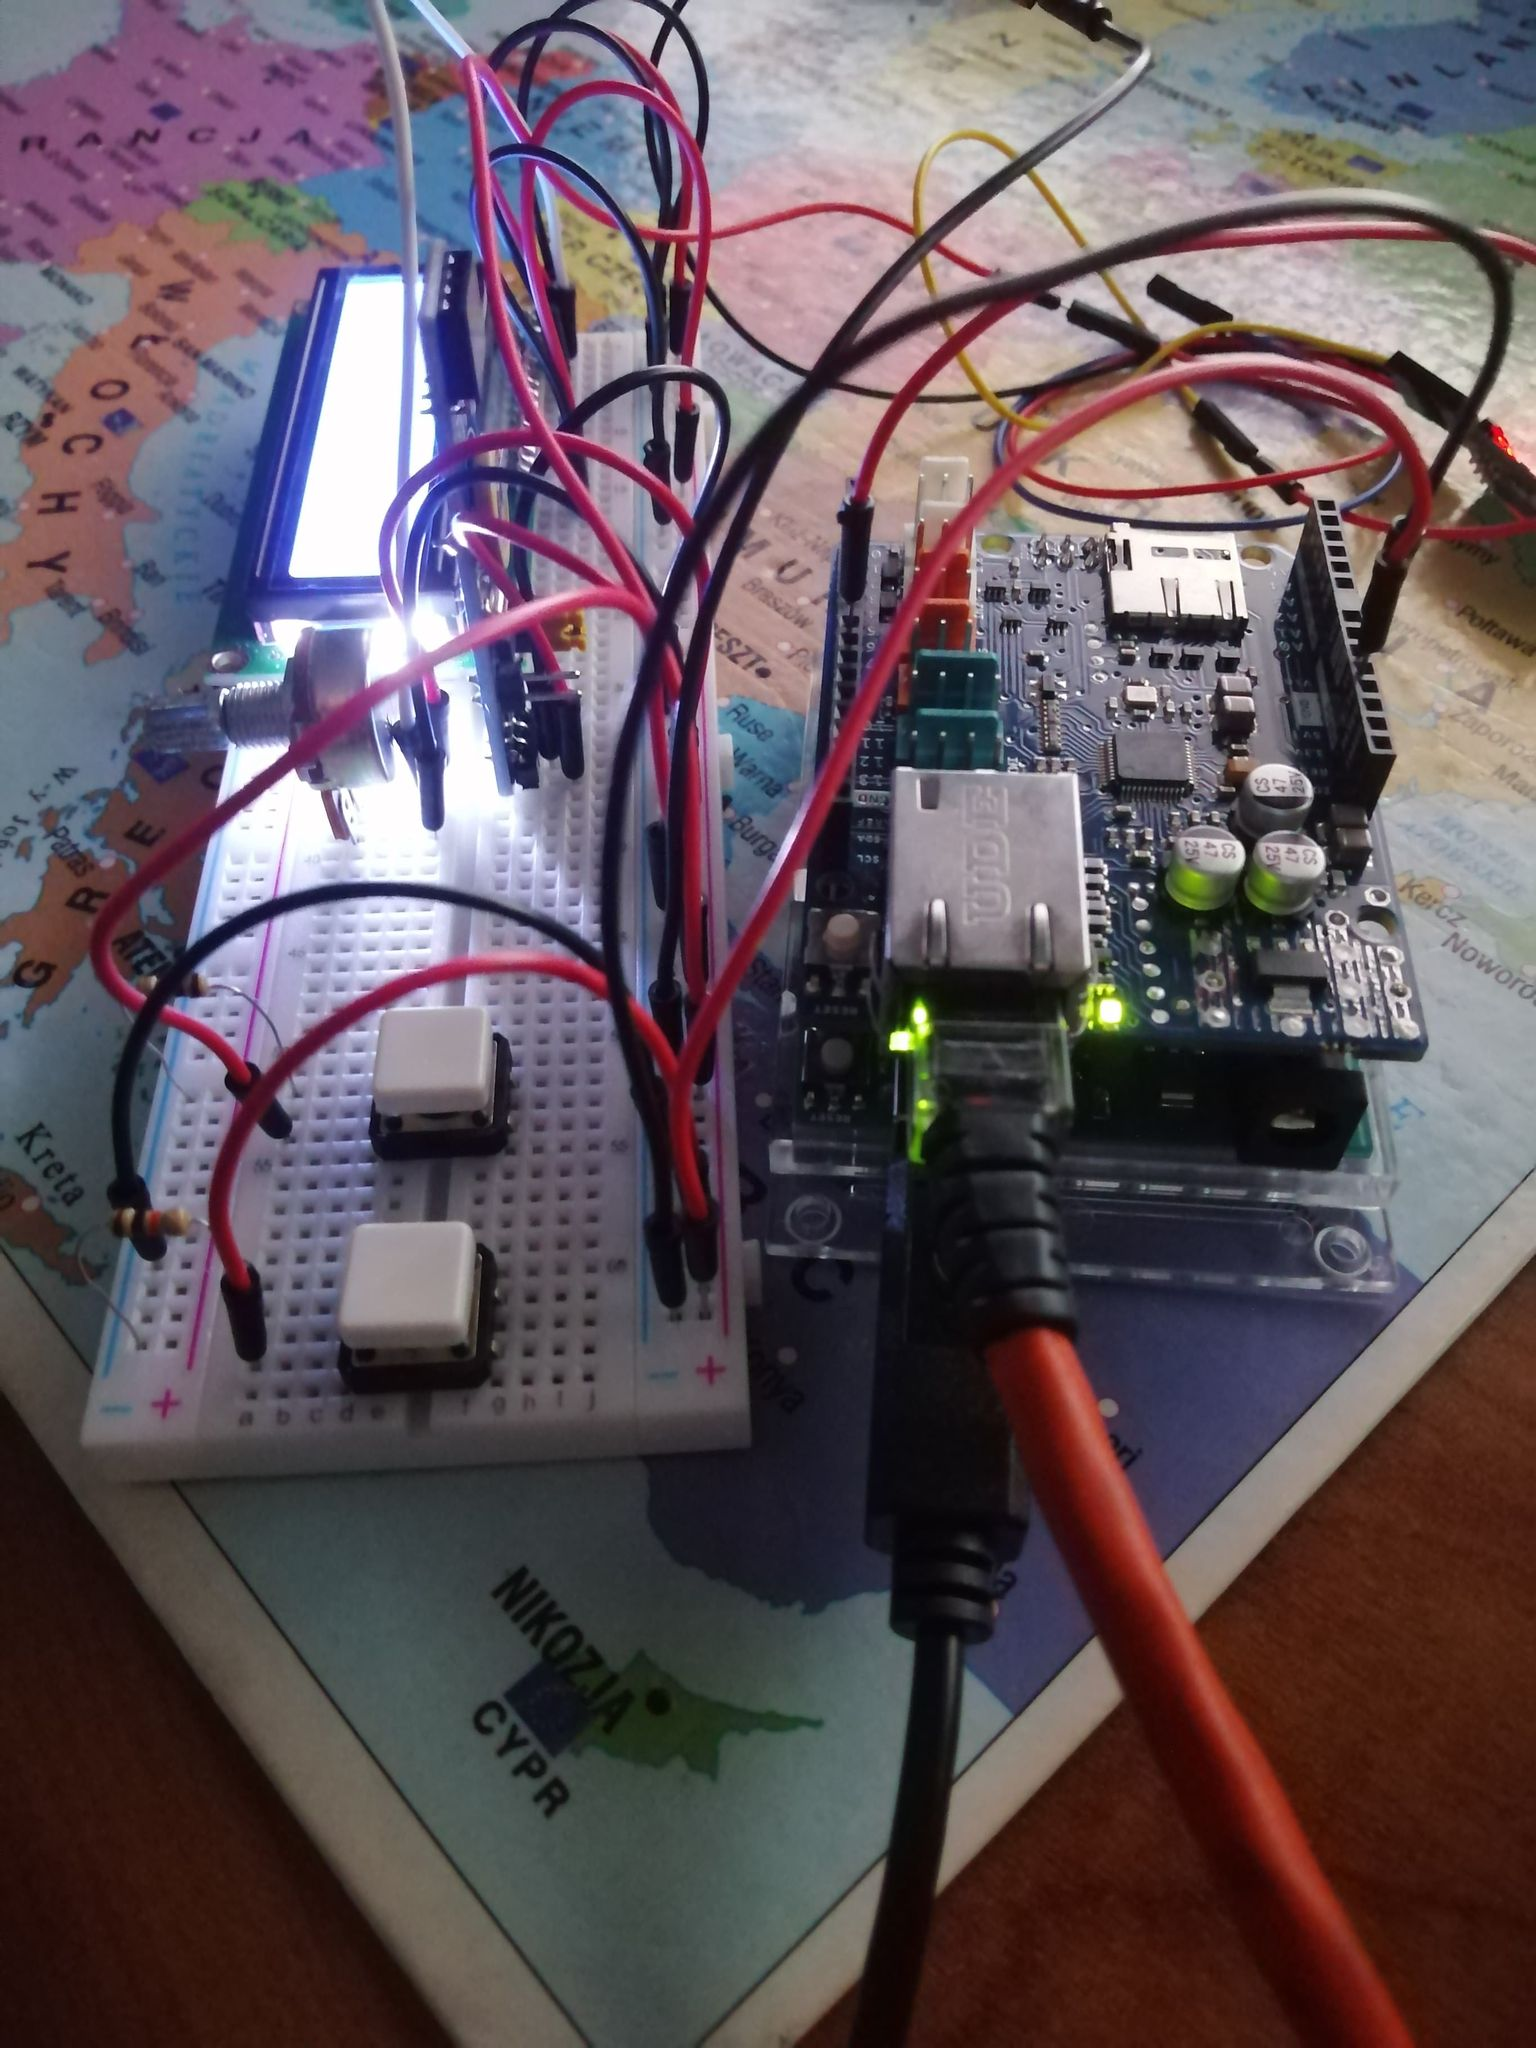
\includegraphics[width=5.0in]{mojuklad.jpg}
	\caption{My arrangement.\label{fig:Myarrangement}}
\end{figure}
\begin{figure}[!b]
	\centering
	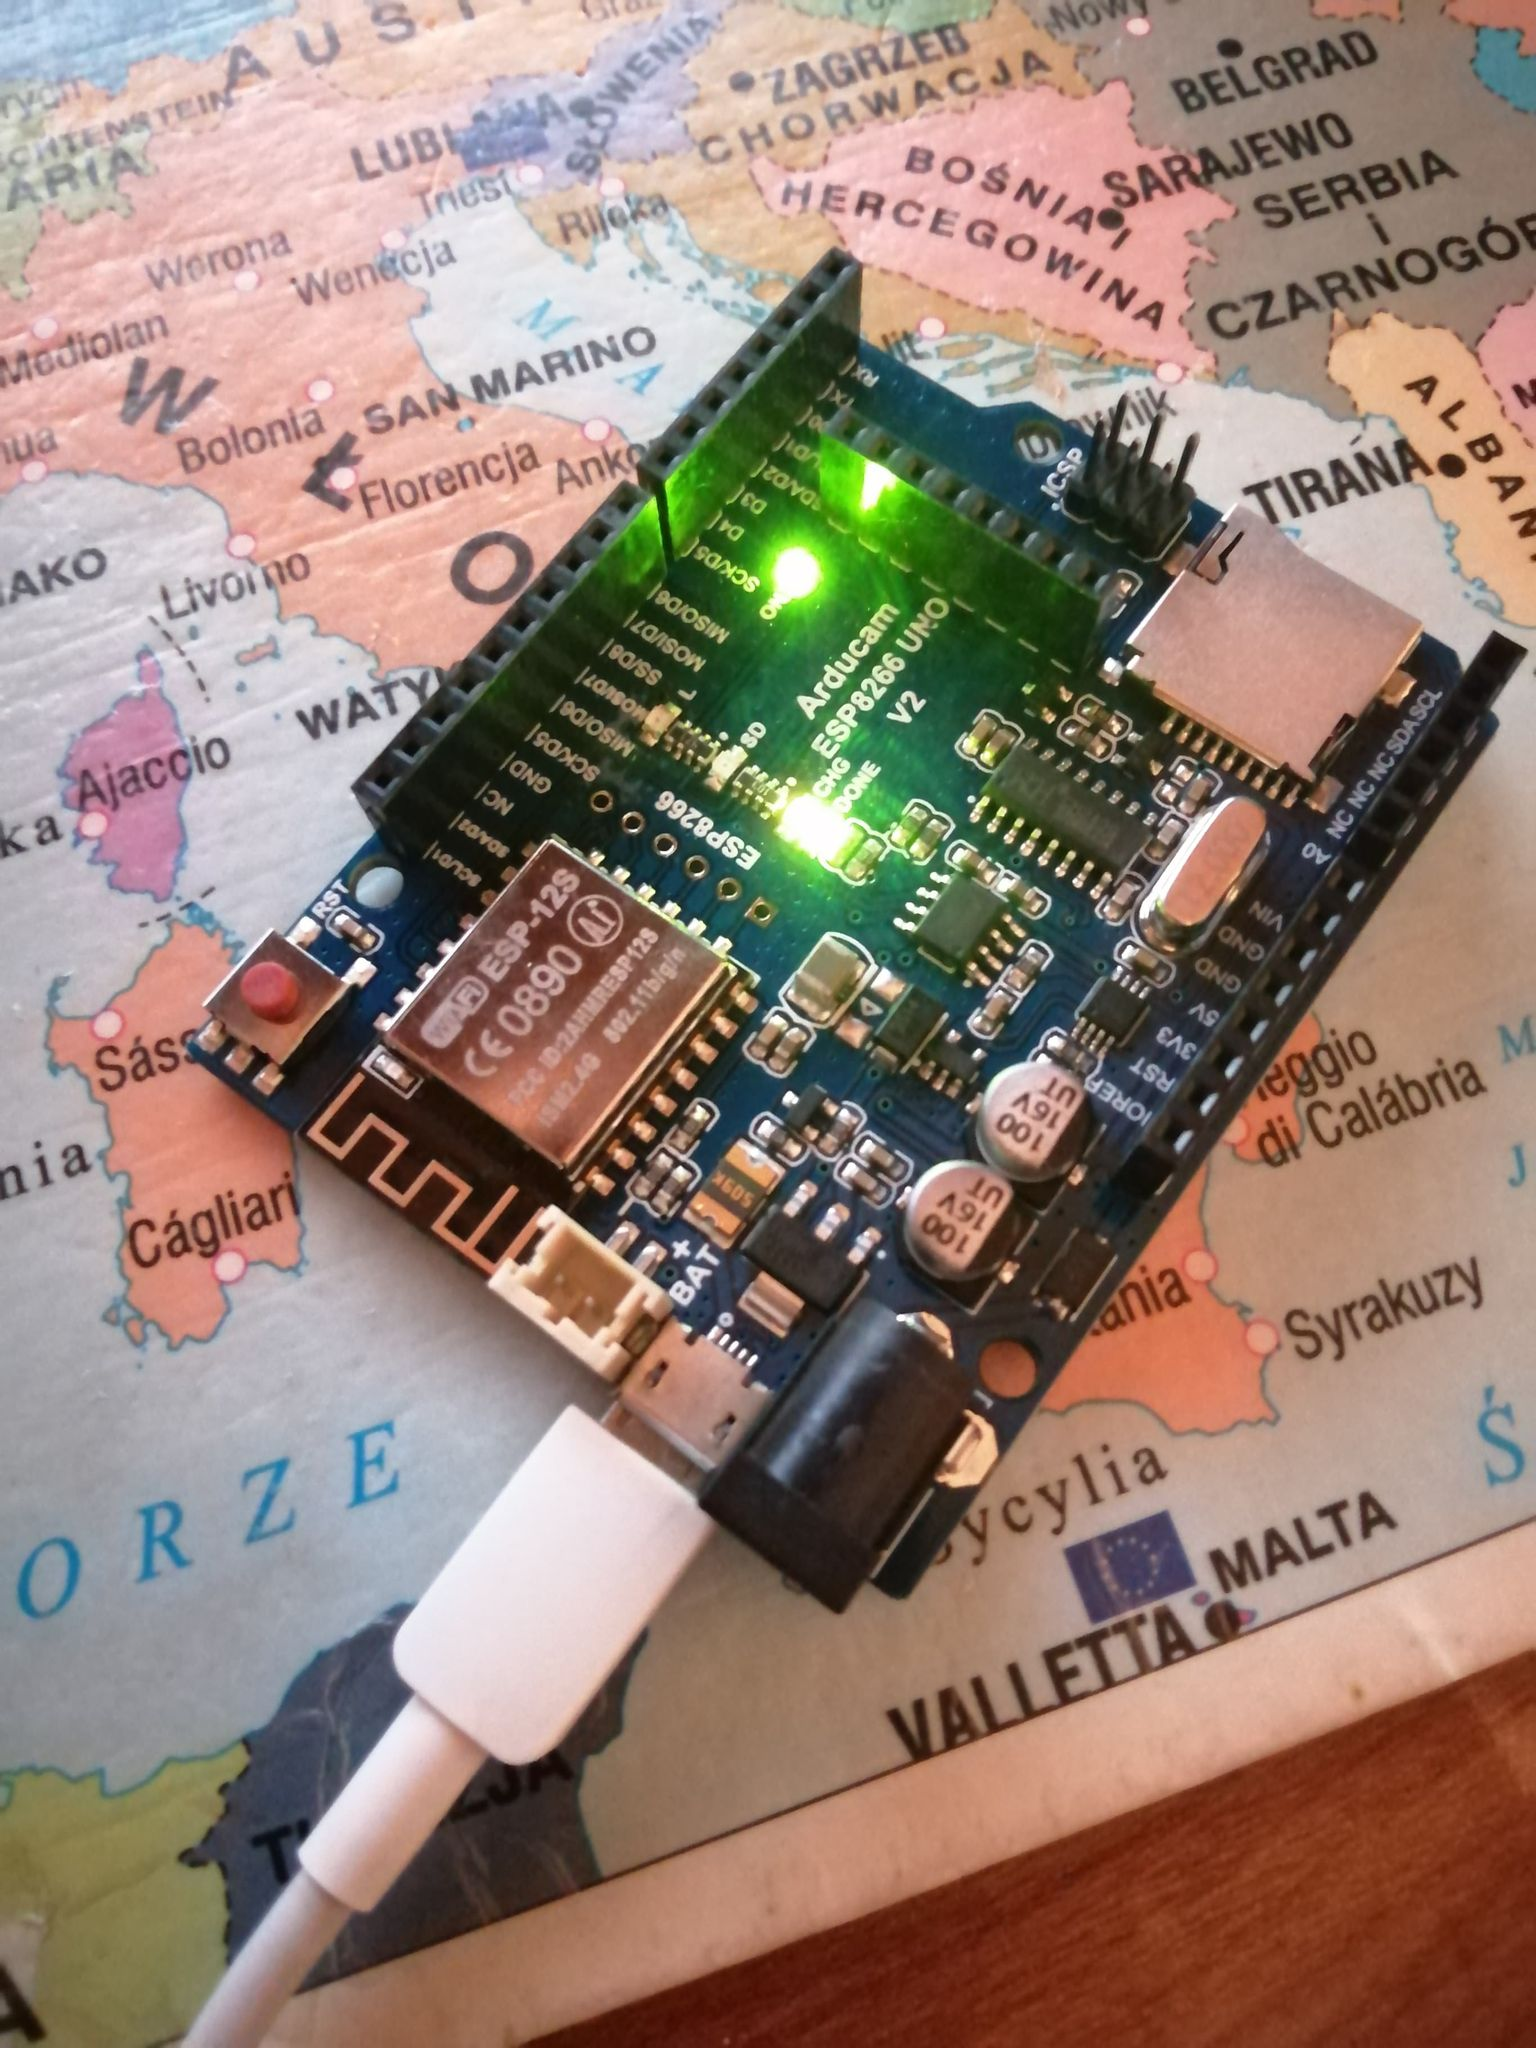
\includegraphics[width=5.0in]{arducam.jpg}
	\caption{arducam.\label{fig:arducam}}
\end{figure}